% Implementation chapter continued
\section{Internals}\label{internals}
\subsection{RabbitMQ as a Central Message Bus}\index{RabbitMQ as a Central Message Bus}
\begin{figure}[h!]
  \centering
  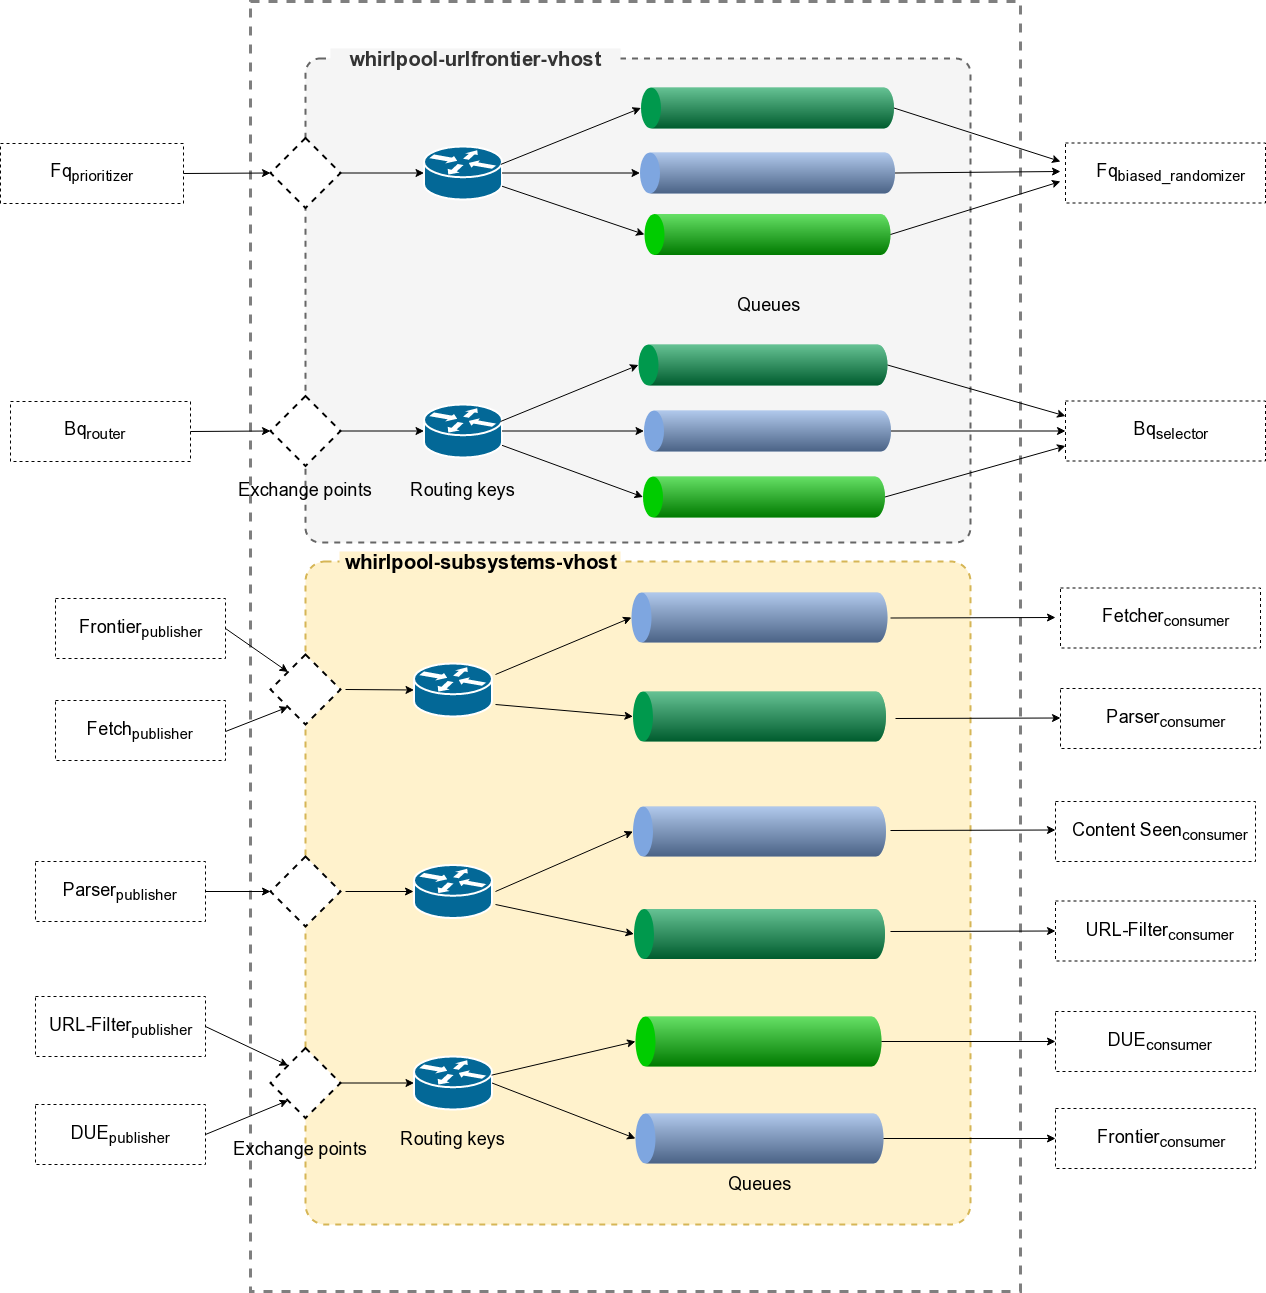
\includegraphics[width=20cm,height=15cm,keepaspectratio]{../media/crawler/rmq-broker.png}
  \caption{Message Distribution using RabbitMQ Direct Exchange}
  \label{fig:rmq}
\end{figure}

\noindent
The initial rabbitmq configuration is shown in the \url{https://github.com/rihbyne/whirlpool-rmq/blob/master/setup.j}. The subsystems only need to know the exchange points and submit message payload to it. The exchange points take care of routing payload to its recipient queue. The payload is static, and doesn't contain any business logic, this leaves the subsystems highly decoupled from each other.
\pagebreak

\subsection{Shared Services with Docker}\index{Shared Services with Docker}
\begin{figure}[h!]
  \centering
  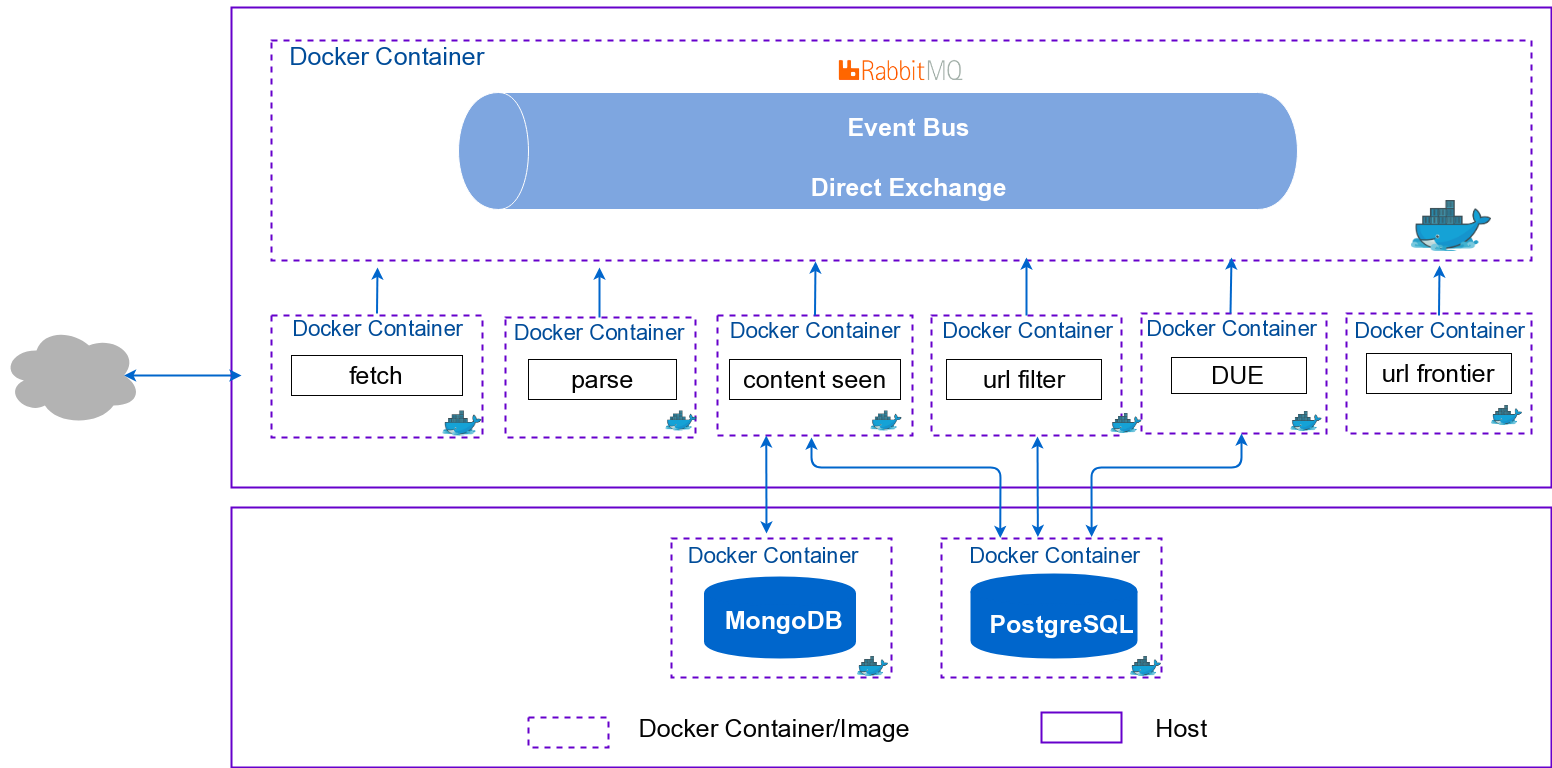
\includegraphics[width=18cm,height=10cm,keepaspectratio]{../media/crawler/multi-container-deploy.png}
  \caption{Single-node Whirlpool Subsystem Isolation using Docker}
  \label{fig:multicontainer}
\end{figure}

\pagebreak

\subsection{Developing with Docker}\label{devdocker}
showcase a dev docker setup(docker-compose.build.yml)

%\inputminted[
%fontfamily=tt,
%baselinestretch=1.2,
%fontsize=\footnotesize,
%linenos,
%breaklines,
%numbersep=5pt,
%tabsize=2,
%frame=single]{js}{../../whirlpool/crawler/whirlpool-user-iam-ec2-vpc-policy.json}


\pagebreak

\subsection{Parser \& its Crawl Ordering Problem}\index{Parser \& its Crawl Ordering Problem}
\begin{figure}[h!]
  \centering
  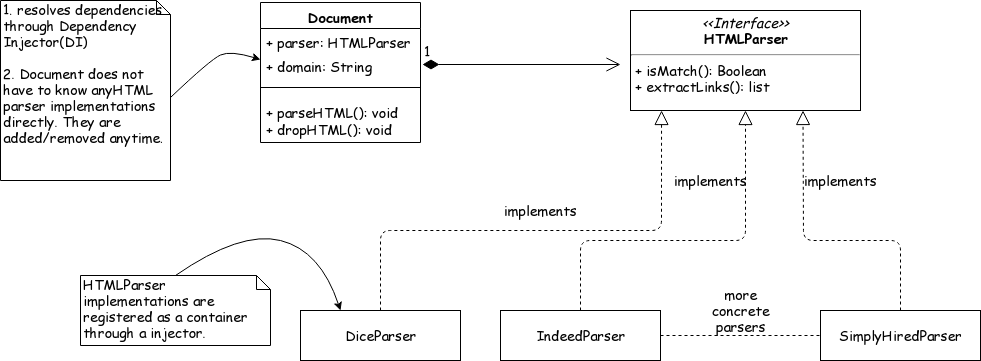
\includegraphics[width=15cm,height=12cm,keepaspectratio]{../media/crawler/docparsers.png}
  \caption{Whirlpool Parser subsystem using Dependency Injection}
  \label{fig:htmlparser}
\end{figure}

\pagebreak

\subsection{URL filtering algorithm}\index{URL Frontier}
\subsection{URL Frontier}\index{URL Frontier}
\subsubsection{Prioritizer Policy}\label{priotizer}
\subsubsection{Front Queue Biased Selection Policy}\label{fqbiased}
\subsection{Distributing the crawl(Linear vs. Consistent Hashing)}

\pagebreak